\documentclass[11pt]{article}
\usepackage{epsfig}

\pagestyle{plain}
\textwidth 17cm
\textheight 23.4cm
\oddsidemargin -12pt
\topmargin 0pt


\begin{document}

\centerline
{\Large \bf MINI-HOW-TO }

\vspace{4cm}

\centerline
{\Large \bf {\sc \Huge mocassin} Version 2.02 }

\vspace{2cm}

\centerline
{\Large (MOnte CArlo SimulationS of Ionized Nebulae) }


\vspace{3cm}

\centerline
{LAST MODIFIED: 19/09/2008}



\vspace{10cm}



\centerline
{\bf barbara ercolano, harvard-smithsonian centre for astrophysics,
  cambridge, ma} 

\vspace{10cm}


\vspace{0.7cm}

\pagebreak

\noindent{\large CONTENTS}\\
\\
\noindent {0. What's new}\\
\noindent {1. How to get MOCASSIN up and running}\\
\indent
    1.1 Obtaining the MOCASSIN source code\\
\indent
    1.2 Unpacking the tarball\\
\indent
    1.3 Compiling mocassin, mocassinWarm mocassinOutput or mocassinPlot\\
\indent
    1.4 Writing a new Makefile\\
\\
\noindent 2. How to run the benchmark cases\\
\indent
    2.1 Pure photoionisation benchmarks\\
\indent        ~~2.1.1 The benchmark problems\\
\indent        ~~2.1.2 Input files for benchmarks\\	
\indent        ~~2.1.3 Running a MOCASSIN pure photoionisation benchmark\\
\indent        ~~2.1.4 Checking everything is going OK\\
\indent        ~~2.1.5 Completing the benchmark runs\\
\indent        ~~2.1.6 Comparing with the benchmark tables\\
\indent 2.2 Pure Dust Benchmarks\\
\indent        ~~2.2.1 1D Benchmarks\\
\indent        ~~2.2.2 2D Benchmarks\\
\\
\noindent 3. Running things other than benchmark cases\\
\indent    3.1 List of keywords\\
\\
\noindent 4. Input and Output Files\\
\indent    4.1 Input files\\
\indent    4.2 Output files\\
\\
\noindent 5. Miscellaneous notes on MOCASSIN\\
\indent 5.1 Analytical and Monte Carlo line fluxes\\
\indent 5.2 Running multiple spatial grids\\
\indent 5.3 Running models that include dust and gas\\
\indent 5.4 The accessories/ subdirectory\\
\indent 5.5 Plotting dust temperatures\\
\indent 5.6 Grain temperature spiking procedures\\
\\
\noindent 6. Limitations and future development\\

\pagebreak

\noindent{\bf \large 0. What's new}\\
\\
\paragraph{from 2.02.54 to 2.02.53} Back to old atomic data. (problems with formats)
\paragraph{from 2.02.52 to 2.02.53} Updated atomic data to Chianti 6. Also added NiII and CaII from the forthcoming Chianti 7. Changed the SED.out output to give flux in Jy multiplied by D$^2$ where D is in pc (users must divide by D$^2$ to obtain flux in Jy. Reinstated the accessories directory with a plotSED.pro idl program included. Echo keyword included - see list of keywords below. 
\paragraph{from 2.02.51 to 2.02.52} Fixed bug in mocassinWarm and mocassinOutput in grid\_mod and fixed but that affected plane parallel models.
\paragraph{from 2.02.50 to 2.02.51} Fixed bug in mocassinOutput mocassinWarm
\paragraph{from 2.02.49 to 2.02.50} 2D option implemented. Does not work with multigrids. 
\paragraph{from 2.02.48 to 2.02.49} removed the tau.out output, now mocassin produces tauNu.out output, which is the tau(nu) at the edge of the grid in the three axial directions starting from the origin of the axes. 
\paragraph{from 2.02.47 to 2.02.48} removed bad Chianti data and reformatted data comments to be more portable.
\paragraph{from 2.02.46 to 2.02.47} the lgIsotropic option is now carried through to the mocassinWarm start routine
\paragraph{from 2.02.45 to 2.02.46} added unisotropic scattering - the <cos theta>  are calculated directly from the dielectric constants through MIE theory and make use of the Heyney Greenstein  phase function - polarisation not included but would be trivial at this point. Isotropic scattering case is still available via the inclusion of the keyword isotropicScattering
\paragraph{from 2.02.44 to 2.02.45} fixed bug that caused mocassin to 
hang after convergence has been reached
\paragraph{from 2.02.43 to 2.02.44} fixed bug in HeI rec lines routine
(extrapolation beyond atomic data temperature limits caused
inappropriate He I recombination line ratios- only affected HeI
recombiation line estimates for model with a significant number of
cells with Te< 5kK). Bug affected versions 2.02.31-2.02.42.
\paragraph{from 2.02.42 to 2.02.43} fixed bug in nu searching routine
(caused spikes in SED when resolution changed dramatically)
\paragraph{from 2.02.41 to 2.02.42} fixed bug in dust PDF calculations
\paragraph{from 2.02.40 to 2.02.41} fixed bug in Lphot->Lstar
conversion for dust+gas simulations
\paragraph{from 2.02.39 to 2.02.40} fixed bug in HeI rec lines routine
\paragraph{from 2.02.38 to 2.02.39} fixed allocation bug in update -
grain heating - only affected g-fortran; fixed bug affecting multistar
models in symmetricXYZ run for only 1 source not centtrally located
\paragraph{from 2.02.37 to 2.02.38} g-fortran compatible
\paragraph{from 2.02.36 to 2.02.37} nForLevels can be used for FeII 
\paragraph{from 2.02.35 to 2.02.36} bug fixed in statistical weightsoutshells affecting species with z>18
\paragraph{from 2.02.34 to 2.02.35} bug fixed in reading PAH files
\paragraph{from 2.02.33 to 2.02.34} bug fixed in mocassinPlot
\paragraph{from 2.02.32 to 2.02.33} HeI recombination lines routine fixed in emission\_mod and output\_mod.
\paragraph{from 2.02.31 to 2.02.32} bugs fixed in output\_mod - recombination contribution to forbidden transitions added to selected ions - ci.dat    ciii.dat  neiv.dat  nev.dat   ni.dat    nii.dat   niv.dat   oii.dat   oiii.dat (W. Wei, Hai Bo - PKU); equilibrium routine and its calls also changed accordingly; to see what CELs now include the recombination contributions please see the end of the data/*.dat files listed. 
\paragraph{from 2.02.30 to 2.02.31} HeI recombination line data modified to include density dependancy.
\paragraph{from 2.02.29 to 2.02.30} forbiddenlines pointers modified.
\paragraph{from 2.02.28 to 2.02.29} bug fixed with mocassinPlot.
\paragraph{from 2.02.14 to 2.02.28} some bugs fixed, most regarding the application of multigrids and of multiple ionisation sources. Previous syntax for multigrids and multiple sources is obsolete. Please check relevant sections. New autmatic contShape allowed {\it powerlaw}. Plane ionisation cases: energy threshold option introduced -- see planeIonization. New keywords: {\it nstages}, {\it getEquivalentTau}.
\paragraph{from 2.02.12 to 2.02.14} diffuse ionisation source included see diffuseSource keyword. V 2.02.13 was skipped as it includes extinction map routines - redundant - and also it has a higher number of Hlevels so it runs slower. 

\paragraph {from 2.01 to 2.02}  ionising stellar atmosphere files from  http://astro.uni-tuebingen.de/~rauch can now be directly read into MOCASSIN (but please manually remove the header). Grain charge calculations. Photoelectric heating from dust grains. Gas-grain collisions. Tspiking. 
PAH optical constants included. Dust optical constant data can be entered in terms of Qs (lambda dependent and radius dependent).
Please refer to {\it Input file} section of this manual. \\
See changes to keyword: {\it contShape}\\
See new keywords: {\it traceHeating}, {\it quantumHeatGrain}, {\it quantumHeatGrainParameters}, 
{\it noPhotoelectric}
\\
\paragraph {from 2.00 to 2.01} The main changes regard the introduction of multiple ionising sources placed at any 
location in the grid. See section 3.1 {\it multiPhotoSources}. \\
The central star(s) parameters are now written to a separate output file (output/photoSource.out). \\
This version is fully compatible with inputs of Version 2.00, but not with the grid*.out files (so mocassinWarm compiled with Version 2.01 will not work with grids produced by Version 2.00).\\

\noindent{\bf \large 1. How to get MOCASSIN up and running}
\\
\\
\noindent{\large 1.1 Obtaining the MOCASSIN source code}\\
   We have decided that MOCASSIN's source code will now only be available on
   request by sending an email to Barbara Ercolano (be@star.ucl.ac.uk). The 
   reason for this is that we would like to have an idea of who is using the
   code, making it easier to provide info and new versions and, most importantly,
   should bugs emerge later on, also provide patches. If you have previously 
   downloaded Version 1.01 or earlier, please email me to obtain the new version. \\
\\   
\noindent{\large 1.2. Unpack the tarball}\\
\noindent ~~~    gunzip mocassin.X.XX.tar.gzip\\
\noindent ~~~    tar xvf mocassin.X.XX.tar\\
\\
   This will create the subdirectory mocassin.X.XX and all the files will be put 
   there.\\
   The following subdirectories will also be created:\\
\\
\noindent ~~~    mocassin.X.XX/source     $\rightarrow$ source code for all the modules\\
\noindent ~~~    mocassin.X.XX/input      $\rightarrow$ where mocassin looks for the input files for the 
                               current simulation \\
\noindent ~~~    mocassin.X.XX/output     $\rightarrow$ where mocassin writes the output files \\
\noindent ~~~    mocassin.X.XX/benchmarks $\rightarrow$ input and output files from the benchmark tests \\
\noindent ~~~    mocassin.X.XX/data       $\rightarrow$ containing all atomic data files needed by mocassin \\
\noindent ~~~    mocassin.X.XX/dustData   $\rightarrow$ optical constants library and other dust data files \\
\noindent ~~~    mocassin.X.XX/examples   $\rightarrow$ some examples input files\\
\noindent ~~~    mocassin.X.XX/accessories$\rightarrow$ miscellaneous FORTRAN and IDL programs\\
\\
\noindent{\large 1.3. Compile mocassin, mocassinWarm, mocassinOutput or mocassinPlot}\\
   In the tar ball you should find an example makefile;
   this was coded for use with the current free Intel F90 compiler 
   (ifort 8.0.034) and the standard free MPI libraries (mpich-1.2.5.2)
   Please edit the makefile to suit the path of the  compiler and mpi libraries on
   your system. some compilers may require different/additional optimisation flags.   \\

   Several other makefiles created for a number of different platforms are also included
   (e.g. makefile.sun etc..); these are only given as further examples and are not 
   being mantained.\\

   Whatever you do PLEASE be careful with aggressive optimization switches. -O5 seems to work fine on all platforms
   so far, but -fsimple=2 gives serious problems. {\bf ALWAYS RUN A BENCHMARK CASE WHEN COMPILING ON A NEW PLATFORM!!}.

   There are four drivers for MOCASSIN: \\
\indent    mocassin: the main mocassin driver that is used to start a new simulation.\\
\indent    mocassinWarm: the driver that is used to resume an interrupted simulation.\\
\indent    mocassinOutput: runs the output routines using the current grid files in the output subdiretory.\\
\indent    mocassinPlot: uses the current grid files in the output/ subdirectory to create 3d-emission maps. \\

   To compile either of these drivers you need to do type:\\
\\
\indent     make mocassin\\
\indent     make mocassinWarm\\
\indent     make mocassinOutput\\
\indent     make mocassinPlot  \\

   WARNING!!!! Sometimes (e.g. on the SUN) the makefile is such that you have to type \\
\\
\indent     make \\

\noindent   first, this will make all the object files, then to link up one of the 
   versions of the driver listed above type\\
\\
\indent     make mocassin \\
\indent     make mocassinWarm\\
\indent     make mocassinOutput\\ 
\indent     make mocassinPlot\\

\noindent   .... if no compiler errors and everything has gone smoothly then the sun will shine and 
   all will be very nice.. if you get compilation errors please email them me them 
   (be\@star.ucl.ac.uk) and I will try to help if I can.\\

\noindent   IMORTANT NOTE: If you are using an IBM platform and the makefile provided here
   then you will also need to change all the module file extensions from 
   .f90 to .f (this is because for some annoying reason the compiler only 
   looks for .f files.. I am sure there must be a way around this, but I 
   couldn't find it, if you do, please let me know!). The file extensions can
   be easily changed using the following single line awk command: \\
\\
\indent     ls *.f90 | awk 'gsub("90",""){print"mv "$1"90 "$1}' | sh\\
\\
\noindent{\large 1.4. Writing a new Makefile}\\
   MOCASSIN's source code is identical for all platforms, only the
   makefile  changes. To write a new makefile a good place to start is
   to find out what Fortran 90 compiler is installed on your machine
   and then read the compiler's man pages.  e.g. if you are using
   xlf90, then just type  man xlf90  and read all the available
   compiler options. You will need to include some  sort of
   optimisation flag and some other MPI related flags. You can refer
   to the makefiles given here for the other platforms.\\

\pagebreak

\noindent{\bf \large 2. How to run the benchmark cases}\\

\noindent{\large 2.1 Pure photoionisation benchmarks}\\

\noindent 2.1.1  The benchmark problems\\
        Once you have downloaded, unpacked and compiled MOCASSIN successfully you can 
        first of all try to run one or more of the available benchmark problems. These 
        were designed at a series of workshops on photoionised plasma codes held 
        at Meudon (France) and Lexington (USA). The latest version of these benchmarks
        are included in Pequignot et al. (2001) in Spectroscopic Challenges of 
        Photoionised Plasmas, ASP Conference Series Vol 247; G. Ferland and D.W. Savina
        eds. Should these conference proceedings not be available to you, the same 
        benchmarks are also reported in Ercolano et al., 2003, MNRAS, 340, 1136. 
        Here you will also find some more general info about MOCASSIN. 
        (There is also a link to this paper at www.star.ucl.ac.uk/~be, following the 
        refereed journal papers link).
	Please note that the MOCASSIN results included in the Pequignot et al. (2001)
	were only from a very early version of the code. Best results are those 
	listed in the Ercolano et al., 2003, MNRAS, 340, 1136 paper.\\


\noindent 2.1.2 Input files for benchmarks\\
        Copy the input file of the benchmark you wish to run (you should have 
        found these in a subdirectory called benchmarks, also included in the tar ball) 
        into the mocassin.X.XX/input subdirectory and rename it input.in or link the input.in 
        file to the benchmark file.\\
    
\noindent        e.g. for the Meudon standard HII region ($T_{\rm star}$=40kK) (assume MOCASSIN 
        is in ~/mocassin.X.XX/ ) type\\
\indent  cp ~/mocassin.X.XX/benchmarks/gas/HII40/meudonHII40.in ~/mocassin.X.XX/input/input.in \\
       or \\
\indent  ln -s ~/mocassin.X.XX/benchmarks/gas/HII40/meudonHII40.in ~/mocassin.X.XX/input.in\\

\noindent also copy the respective nebular abundance file into the same directory (no 
        need to rename!). In the case of the Meudon standard HII region benchmark 
        this will be abunHII40.in (you can check the name of the abundance file, 
        which is given in the input.in file with keyword nebComposition)\\
\indent  cp ~/mocassin.X.XX/benchmarks/gas/HII40/abunHII40.in ~/mocassin.X.XX/input/abunHII40.in\\
\\
\noindent 2.1.3 Run a MOCASSIN pure photoionisation benchmark\\
        The command you need to use to actually run MOCASSIN will depend on how your system is 
        set up, and whether you are required to run your models through a queueing 
        system, in which case you will probably need some sort of shell script to do 
        that (ask your network administrator if unsure).
        If you want to run MOCASSIN outside any queueing system then you can try one of 
        the following commands and hope that one works, if not ask you network 
        administrator about how to interactively run MPI programs on your system.\\

\noindent        for the SUN: \\
\indent         mprun -np N ./mocassin   (where N=number of processors you wish to use) \\

\noindent        for the IBM\\
\indent         mocassin -procs N (where N=number of processors you wish to use)\\

\noindent        for the SGI, Beowulf and single Linux PCs using the standard MPI as above:\\
\indent         mpirun -np N ./mocassin (where N=number of processors you wish to use)\indent 

\noindent 2.1.4 Checking that everything is going OK\\
        If the 'output' keyword is included in the input file (see 3.1), 
        at the end of each iteration MOCASSIN will write out a number of output files 
        (see 4.) in the output/ directory. 
        Some of them are written out regardless of whether the 'output'
        keyword is included, these are grid files that are needed by the mocassinWarm 
        driver (should you decide to stop the simulation and re-start it from the same 
        iteration); see 3.1, 'writeGrid' keyword to see how to control the output grid files. 
        Also MOCASSIN will keep you updated on what he is doing by 
        outputting stuff to the screen (if that annoys you, just pipe it to a file 
        e.g. mocassin -procs N $>$ log; and then you can check the log at any time 
        you wish). \\
        After each iteration it will tell you the percentage of grid-cells 
        converged so far, as well as the number of 'dark cells' (i.e. those cells not reached
        by any of the photon packets) and also will provide a summary of eventual 
        convergence problems generally this is the last bit of info written before the 
        beginning of the new iteration, so, if you have decided to pipe the screen output
        into a file called log, then you can easily check the progress so far by 
        typing tail -f log, or grep Summary log, or more simply, the convergence history is 
	summarised in a file called 'output/summary.out.  \\
        For the benchmark cases you can start having an idea of whether MOCASSIN is working 
        properly by waiting until it's about 60-70\% converged and 
        then checking the 'output/lineFlux.out' file. A description of this file is 
        given in section 4. of this README file. Also check the 'output/temperature.out' and
        the 'output/ionratio.out' files (also described in section 4.).\\

\noindent 2.1.5 Completing the benchmark runs\\
        The benchmark input files included are set up to run a simulation of 
        13*13*13 grid cells (this is sufficient to reproduce the benchmark results; see 
        Ercolano et al., 2003) and a given starting number of energy packets 	
        (e.g. this can be set by the keyword nPhotons 100000); 
        one iteration of 100000 packet should run in a few minutes on most systems.	
        The benchmarks input files make use of the Autopackets option (see 3.1), which 
        which automatically increases the number of energy packets to be used as soon as
        a convergence plateau is reached. \\
        This could also be done manually, by excluding the Autopackets option from the input 
        file and starting off with about 1000000 packets.
        However 1000000 photons are not enough to reach full convergence in this case 
        and you will have to stop the simulation when the percentage convergence reaches 
        30-40\%, then edit the grid3.out file changing 1000000 to 3000000, and restart the 
        simulation using the previously compiled mocassinWarm driver \\
\indent  e.g. mprun -np N ./mocassinWarm\\
\noindent        this will basically tell MOCASSIN to increase the number of energy packets 
        to be used in the simulation from 1000000 to 3000000. It will, of course, 
        now take longer to complete each iteration, but the convergence percentage 
        should increase quite quickly. You can stop the simulation when you reach 
        convergence $>$ 90\%. 
        For simplicity, until you familiarise yourself with the program, it is advised 
        that you keep the Autopackets option as set in the input files, 
        in which case it will not be needed to manually stop and restart the simulation.\\

\noindent 2.1.6 Comparing with the benchmark tables\\
        The description of the output files is given in section 4. The output files
	contain all the info (and much more) you need to compare your simulation with 
        the benchmark tables. Remember that MOCASSIN employs a statistical method, so
        do NOT expect to see exactly the same figures as those quote in the benchmark
        paper as some of the differences will be due to the statistical error and also 
        to the convergence level/limit employed. Furthermore some of the atomic data
        has been updated since the publication of the paper. \\

\noindent{\large 2.2 Pure Dust Benchmarks}\\
   Version 2.0 was designed for the modelling of regions where dust grains and photoionised 
   gas coexist in the same volume; however extreme care has been taken so that the code 
   could also be run efficiently when only one or the other process is included. 
   In this section we will see briefly how to run dust-only models by attempting to 
   reproduce pure dust 1D and 2D models as shown by Ercolano, Barlow and Storey 
   (2005, MNRAS, in press). \\

\noindent 2.2.1 1D Benchmarks\\
       A set of spherically symmetric benchmark models and solutions are described by 
       Ivezic et al. (1997, MNRAS, 291, 121). 
       The input files used by MOCASSIN for some of these benchmarks are included in 
       the directory ~/mocassin.X.XX/benchmarks/dust/1D. \\
       Copy the input file of the benchmark you wish to run  
       into the mocassin.X.XX/input subdirectory and rename it input.in or link the input.in 
       file to the benchmark file. Then run the code (see Section 2.1.3) and finally 
       compare the output files (SED.out dustGrid.out, see Section 4) with the results 
       published by Ercolano, Barlow and Storey (2005, MNRAS, in press)\\
     

\noindent 2.2.1 2D Benchmarks\\
       A set of 2D disk benchmark models and solutions are described by Pascucci et al. 
       (2004, A\&A, 417, 793).
       Sample input files used by MOCASSIN for some of these benchmarks are included in 
       the directory ~/mocassin.X.XX/benchmarks/dust/2D. \\
       As for the 1D benchmarks you will have to copy the input files of the 
       benchmark you wish to run  
       into the mocassin.X.XX/input subdirectory and rename it input.in or link the input.in 
       file to the benchmark file. Then run the code (see Section 2.1.3) and finally 
       compare the output files (SED.out dustGrid.out, see Section 4) with the results 
       published by Ercolano, Barlow and Storey (2005, MNRAS, in press).\\

\pagebreak 

\noindent{\bf \large 3. Running things other than benchmark cases} \\

   Once you have convinced yourself that MOCASSIN is behaving as it should, you 
   can run your own simulations. If you are not confident that this is the case, 
   please contact me before going any further. \\
   
   The first step is to define your model. This is done via a set of keywords 
   included in the input.in file. YOU SHOULD NEVER HAVE TO CHANGE ANYTHING IN THE
   SOURCE CODE (I hope). If you find you have to, please let me know.
   The rest of this section will list and describe all the keywords that can be 
   included in the input file. The number of keywords you decide to use and the 
   order you decide to list them in is entirely up to you. If you have missed out
   some required and fundamental keyword the simulation will stop and tell you what 
   you have missed out. However, you should be aware that, for most of these 
   keywords, default values are defined, so make sure that the default value is 
   actually what you want before you decide to leave a given keyword out. Default 
   values to each keyword are given below, enclosed by square brackets. 
   The fundamental keywords, which must be specified in every input file are marked 
   by an asterisk in the square brackets and have no default value. \\

\noindent{\large 3.1 List of keywords}
\paragraph   {autoPackets} real1 real2 integer3: The number of energy packets to be used in the next 
                     iteration will automatically be increased by a factor of real2
		     whenever a convergence plateau (defined by real1) is reached, i.e. 
		     if the convergence level increase is less than the value specified
		     by the user in real1. For example autoPackets 0.10 5. 1e8 will cause 
		     the total number of energy packets to increase by a factor of 5. 
		     whenever the convergence level increase from one iteration to 
		     the other is less than 10\%. This only occurs when the convergence 
		     level is less than 85\% and is the maximum number of packets 
		     defined by integer3 (1e8 in this example) has not been reached.\\
		     $[$.false.$]$

\paragraph {continuumCube} real1 real2 : This keyword creates a 3D cube of the escaped continuum radiation
                     in direction given by the inclination keyword and over all directions. 
		     If no inclination is specified in the input the continuum cube 
		     will include packets escaping in all directions. The continuum band wavelength limits are 		     
                     defined by real1 and real2 (give in $\mu$m). A negative value or the omission of 
		     this keyword will result in no continuum cube being written out. \\
		     $[$-1.$]$		     

\paragraph   {contShape} 'string' [optional: real]: The shape of the ionising continuum. The default value is 
		     'blackbody', in which case the ionising stellar continuum is 
		     approximated by the Planck function for the stellar 
		     temperature defined by the keyword Stellar. If 'string' == 'powerlaw'
		     then this must be followed by a real number indicating the index of the 
		     power law distribution such that $F_{\nu} \propto \nu^{-index}$. E.g. 
		     {\it contShape powerlaw 1. } will generate an input spectrum following a $\nu^{^-1}$
		     distribution. Note that the final result will be normalised to the luminosity entered. 
		     The power law keyword is not compatiblewith the Lphot keyword, but only with the Lstar keyword.
		     If a stellar 
		     atmosphere data file is to be used, the 'string' must specify 
		     the path of the external file containing the data. For example 
		     contShape NLTE140lg65 tells the program to look for the 
		     nLTe140lg65 data file in the current directory. The stellar 
		     atmosphere files must be in a format consisting of two columns:
		     the first listing the wavelength points in units of [A] and 
		     the second containing the corresponding wavelength-dependent 
		     stellar Eddington fluxes in units of $[erg/cm^2/s/A/sr]$. A set
		     of stellar atmosphere flux tables have been compiled by Dr T. Rauch
		     in a MOCASSIN-friendly format and are available  
		     http://astro.uni-tuebingen.de/~rauch/ (but please manually remove 
		     the header from the flux tables.\\
		     $[$blackbody$]$\\

\paragraph   {convLimit real}    : This is the convergence limit for the variation of a given 
                     parameter, in each grid cell from one Monte Carlo iteration to the 
		     next (e.g. 0.05 means changes of 5\% maximum). 
		     In the case of a pure-gas (or gas+dust) simulation the criterion 
		     is based on the rate of change of neutral hydrogen. In the case of 
		     dust-only the criterion is based on the rate of change of the 
		     dust temperatures. 
		     Other convergence criteria can also be used, at the moment, 
		     this would require a simple editing of some source modules. 
		     If you would like to use a different convergence criterion 
		     please email me and I can do the editing for you. \\
		     $[$0.05$]$\\

\paragraph   {debug}             : Logical switch to enable the debugging mode. When this 
		     keyword is included MOCASSIN will calculate a number of 
		     extra quantities (see Section 5.), which will, of course,
		     slow the process down and also require more memory. \\
		     $[$.false.$]$\\

\paragraph   {densityFile 'string'}: The density structure of the nebula can be defined cell by 
	             cell by using an external density file. {\sc mocassin} knows that a 
		     density file is to be used when the densityFile 'string' is 
		     included in the input file, where 'string' contains the name 
		     and path of the file where the data is stored. This file must 
		     be consists of four, five or six columns, with the first three 
		     columns containing the x-, y-, and z- coordinates of the grid cell in 
		     [cm] and the fourth columns containing the value of the hydrogen 
		     density by number in $[cm^{-3}]$ at the particular grid cell. The 
		     x, y and z axis do not to be equally spaces, irregular grids are 
		     perfectly acceptable by MOCASSIN and also the extent of each axis 
		     can vary (as long as this is consistent with the values given in 
		     the nx, ny and nz fields). The fifth column is optional. If the 
                     multiChemistry keyword is specified the fifth column must contain
                     an integer number in the range [1, Ncomponents] which indicates what 
                     component this cell belongs to (so that MOCASSIN can assign the chemical 
                     abundances for this component).\\
		     $[]$\\

\paragraph    {densityLaw real... }: This keyword is usually followed by a set of 
		     parameters which are to be fed into the density law routine, 
		     included in the grid\_mod module. Any density law can be 
		     specified by editing the code in the setGrid subroutine. 
		     If the nebula is homogeneous, this keyword must be omitted 
		     and the Hdensity keyword included instead. Note that if neither
		     of the two keywords is included, and an external density file 
		     is not specified with the densityFile keyword, the nebular 
		     density distribution is left undefined and the simulation 
		     halted with an error message being produced.\\
		     $[$0. 0. etc..$]$\\
    
\paragraph    {dustFile string1 string2} : names dust data files - \\
                     string1 = grain species file\\
                     string2 = grain size info file\\
		     $[$"none", "none"$]$\\

\paragraph{echo real1 real2} : If one needs to account for light travel 
                     time effects, for example if the source luminosity is changing, then this 
                     keyword will cause the results in SED.out to be integrated only over grid 
                     cells lying between ellipsoids corresponding to light travel times of 
                     real1 and real2.  real1 and real2 are in light days, and real1 must be 
                     less than real2.  The ellipsoids open out along the z-axis, and so one 
                     should also specify `inclination 1 0.0 -1' in input.in when using this 
                     keyword.  A review of the geometries of light echoes can be found in 
                     Sugerman, 2003, AJ, 126, 1939, and a case of {\sc mocassin} modelling 
                     including light travel time considerations is described by Wesson et al 
                     (arXiv:0907.0246).\\
                     $[$.false.$]$\\

\paragraph    {edges real1 real2 real3 }: Defines the grid edges (only to be used with automatic
                     grids). real1 real2 and real3 are respectively the x, y and z 
                     edges in cm\\
                     $[$-1., -1., -1. *must be given if automatic grids are used$]$\\
		    

\paragraph    {fillingFactor real1} : real1 can assume all values from 0. to 1. to defines the gas 
                     volume (and/or dust) filling factor\\
                     $[$1.$]$\\

\paragraph    {getEquivalentTau} : Logical switch to enable equivalent optical depth calculations 
(see Ercolano et al. 2007) - useful for diffuse/multiple and non-centrally located ionisation/
illumination sources \\
                     $[$.false.$]$\\

\paragraph    {getTau} : Logical switch to enable optical depth calculations and output - may be 
                     time consuming for large grids\\
                     $[$.false.$]$\\

\paragraph    {Hdensity real }   : This keyword specifies a constant hydrogen density, 
		     by number, throughout the nebular region 
		     The command Hdensity 300 will e.g. set the 
		     hydrogen density, by number, to the constant value of 300 $cm^{-3}$.\\
		     $[$0.$]$\\

\paragraph    {inclination integer real\_1, real\_2 ..... real\_{n1}, real\_{n2}} : This keyword controls the
                     viewing angles at which the SED will be calculated as it will appear 
		     in the SED.out file (see Section 4.2). The number of viewing 
		     angles is given first (integer; in this version integer <= 2) and then the $\theta$
                     and $\phi$ inclination in radians. To turn off the $\phi$ dependence, real\_2 must be set to 
		     to -1. . 
		     ($\theta$ =0. when the line of sight coincides with the z-axis)\\
		     $[$0$]$\\

\paragraph    {inputNe  }        : This indicates that the density distribution of the grid is in 
                     terms of electron densities instead of H density. This will cause 
                     the code to calculate at each iteration the values of H density 
                     from the local Ne values by taking into account the local 
		     ionisation structure. \\
		     $[$.false.$]$\\
\paragraph    {isotropicScattering} : This keyword activates the logical switch that turns off unisotropic scattering 
                     (implemented via the Heyney-Greenstein phase function - with <cos theta> calculated from the dielectric 
                      constants via MIE theory).\\
		     $[$.false.$]$\\                      
\paragraph    {LPhot real	  }   : This is the number of hydrogen-ionizing photons emitted by 
		     the source per unit time, which is generally referred to as 
		     Q(H$^0$), in the literature, with units of [E36 $sec^{-1}$]. If this 
		     is given then the stellar luminosity, LStar is automatically 
		     derived from it.\\
		     $[$* if LStar not given$]$\\

\paragraph    {LStar real}	     : This is the stellar luminosity in units of [E36 erg $sec^{-1}$].
		     If this is given as an input, then the number of hydrogen-
		     ionizing photons,  Q(H$^0$), is automatically derived from it 
		     and from the input spectrum. \\
		     $[$* if LPhot not given$]$\\

\paragraph    {maxIterateMC integer1 real1}: integer1 is the maximum number of Monte Carlo iterations to 
		     be performed in the simulation. real2 is the minimum convergence level
                     to be achieved before the end of a simulation. The program will however 
		     stop after integer1 iteration even if real1\% of convergence has yet to 
		     be reached.\\
		     $[$30 95.$]$\\

\paragraph    {MdMg string1 real1/string2 }: Dust to Gas ratio by mass. If string1 = 'constant' then
                     it must be followed by real1, containing the value of MdMg to be applied 
                     homogeneously to all cells in the grid. If string1=file then it must be 
                     followed by string2, the name of the file defining the MdMg at each 
                     location. Note that MdMg, MdMh and Ndust are mutually exclusive.
                     This file must consists of four columns, with the first three 
		     columns containing the x-, y-, and z- coordinates of the grid cell in 
		     [cm] and the fourth columns containing the dust to gas mass ratio
                     at the particular grid cell. The 
		     x, y and z axis do not to be equally spaces, irregular grids are 
		     perfectly acceptable by MOCASSIN and also the extent of each axis 
		     can vary (as long as this is consistent with the values given in 
		     the nx, ny and nz fields).\\
		     $[$.false. 0./'none'$]$\\

\paragraph    {MdMh string1 real1/string2} : Dust to Hydrogen ratio by mass. If string1 = 'constant' then
                     it must be followed by real1, containing the value of MdMh to be applied 
                     homogeneously to all cells in the grid. If string1=file then it must be 
                     followed by string2, the name of the file defining the MdMh at each 
                     location. Note that MdMg, MdMh and Ndust are mutually exclusive. 
                     This file must consists of four columns, with the first three 
		     columns containing the x-, y-, and z- coordinates of the grid cell in 
		     [cm] and the fourth columns containing the dust to hydrogen mass ratio
                     at the particular grid cell. The 
		     x, y and z axis do not to be equally spaces, irregular grids are 
		     perfectly acceptable by MOCASSIN and also the extent of each axis 
		     can vary (as long as this is consistent with the values given in 
		     the nx, ny and nz fields).\\
		     $[$.false. 0./'none'$]$\\

\paragraph    {multiChemistry integer1 string(1) string(2) ..... string(integer1)}: This keyword must
                     be used when a chemically inhomogeneous model is being performed. 
		     The integer1 value defined the number of components to be used. 
		     string(1), string(2) ... string(integer1) are the names of the 
		     files describing the abundances in each component. 
		     When the multiChemistry keyword is included the density distribution
		     MUST be specified via the densityFile keyword. The fifth column of the 
		     density file must contain the index for the abundance file describing 
		     the chemical composition at each location. \\
		     $[$.false.$]$\\

\paragraph    {multiGrids integer1 string1} : This defines a multiple grid environment. The integer1 is the 
                     total number of grids to be used (mother + subgrids) and string1 
                     is the name of the file containing the subgrid information. 
		     Please see the 'Running multiple spatial grids' section in this 
                     document.\\
                     $[$.false. 'none'$]$\\
                     	   
\paragraph    {multiPhotoSources string1} : This keyword is used to define multiple (or single) ionising sources , that can be placed at any locations. 'string1' is the name of the file containing the central star parameters. This file must contain in the first line the number of sources to be included and then each source should be specified on successive lines providing (in this order) T$_{\rm eff}$ [K], L$_*$ [E36erg/s], ContShape, x-, y-, z-position. Note that the location of the source must be given normalised to the length of the relative axis. As example is included in the example/ directory. \\

\paragraph    {nbins integer  }  : The total number of points to be used in the frequency mesh. \\
		     $[$600$]$\\

\paragraph    {Ndust string1 real1/string2 }: Number density [$cm^{-3}$] of dust grains. If 
                     string1='constant' then it must be followed by real1, containing 
                     the value of Ndust to be applied homogeneously to all cells in the 
                     grid. If string1=file then it must be followed by string2, the name of 
                     the file defining Ndust at each location. Note that MdMg and Ndust are 
		     mutually exclusive. This file must consists of four columns, with the first three 
		     columns containing the x-, y-, and z- coordinates of the grid cell in 
		     [cm] and the fourth columns containing the number density of dust
                     in [$cm^{-3}$] at the particular grid cell. The 
		     x, y and z axis do not to be equally spaces, irregular grids are 
		     perfectly acceptable by MOCASSIN and also the extent of each axis 
		     can vary (as long as this is consistent with the values given in 
		     the nx, ny and nz fields).\\
		     $[$.false. 0./'none'$]$\\

\paragraph   { nebComposition 'string'}: This keyword specifies the path of the nebular 
		     composition data file. If the default 'solar' composition 
		     (defined in the file solar.dat) to be used, this keyword can 
		     be omitted. However the solar.dat file includes all elements 
		     with Z$<$30: this will result in a more memory expensive 
		     simulation. It is therefore advised to set to zero those 
		     elements which are not needed in the simulation. Otherwise the 
		     nebular composition can be specified in the user-defined 'string' 
		     file to be found in the current directory. All composition 
		     input files must be in a format consisting of one column containing 
		     the abundances by number and relative to hydrogen for the first 
		     thirty elements in order of ascending atomic number.
		     The abundances of elements which are not to be included in 
		     the simulations must be set to zero (this will automatically
		     exclude them by flagging them out throughout the program).
		     If the multiChemistry keyword is specified the nebComposition 
		     keyword must be omitted.\\
		     $[$* if gas is present and no multiChemistry$]$\\

\paragraph   { NeStart real   }  : Initial guess for the nebular electron density. \\
		     $[0.]$\\

\paragraph {noPhotoelectric} : When this keyword is included in the input file all procedures associated with the calculation ofthe grain charges and photoelectric yield are switched off as well as gas-grain collision processes. \\
$[.false.]$\\

\paragraph   { nPhotons integer}: This is the number of energy packets to be used in the Monte 
		     Carlo simulation and it has to be specified for each model.\\
		     $[*]$ \\

\paragraph   { nStages integer}: This is the number of ionisation stages to be used in the model.Max allowed is currently 10. If you have the atomic data necessary and would like to use more than 10 ionisation stages please contact me, or if you are confident you can edit the data/fileNames.dat and include the new data files to the poole. \\
		     $[7]$ \\

\paragraph   { nuMax real  }    : High limit of the frequency mesh in units of $[Ryd]$\\
		     $[15.]$\\

\paragraph   { nuMin real }     : Low limit of the frequency mesh in units of $[Ryd]$\\
		     $[0.]$\\

\paragraph   { nx integer }     : Number of axial points in the x-direction.\\
		     $[30]$\\

\paragraph  {  ny integer}      : Number of axial points in the y-direction.\\
		     $[30]$\\

\paragraph  {  nz integer  }    : Number of axial points in the z-direction.\\
		     $[30]$\\

\paragraph  {  output  }        : when this keyword is included the output files will be written
                    at the end of each iteration. If it is omitted no output will be 
		    created, however if the grid files are being created the output 
                    files can easily be recovered using the mocassinOutput driver. \\
                    $[.false.]$\\
		    
\paragraph  {  planeIonization real1 real2} : this keyword is used when the ionisation source is from a 
                    plane and not from a point source. real1 must contain the value 
		    of the incident ionizing flux above nu = real2 [Ryd] (constant at each point on the plane) in units of 
		    [$phot/s/cm^2$]. If real2 =0. then the real1 is assumed to be the bolometric flux. 
		    When this keyword is specified the density distribution
		    must be defined via the densityFile option. The ionizing plane is the 
		    x-z plane. the energy packets are reflected when they hit the y-z and
		    the y-x planes and can escape from the x-z planes. (This can be easily 
		    changed to suit. please contact me be@star.ucl.ac.uk if your work requires 
		    it to be different)\\
		    $[.false.]$\\

\paragraph {quantumHeatGrain real1 real2}: This keyword activated the temperature spiking routines (quantum grain heating). It is only valid for simulations including dust. real1 is the limiting size of grain radii [um] that will be allowed to spike (i.e. grains with a < real1 will spike). real2 is the minimum convergence level for the spiking to occur. Please read the notes on {\it Grain temperature spiking procedures} contained in this manual.\\
$[1.e-3, 99.]$\\

\paragraph {quantumHeatGrainParameters real1 integer1 logical1}: This keyword provides controls over some internal parameters in the quantum grain heating procedures. They should not be modified unless you really know what you are doing.  real1 is the max temperature to be considered in the grain temperature mesh of the spiking. integer1  is the number of temperature (and enthalpy) bins considered. logical1 switches on and off the writing out of a file containing all the probability functions for all the grains in every cell. The resulting file can be really gigantic and so this value should be set to .true. only for debugging purposes and used with care. Please read the notes on {\it Grain temperature spiking procedures} contained in this manual.\\
$[700., 300, .false.]$
 
\paragraph  {  Rin real}	    : Inner radius of the ionised region, in units of $[cm]$.\\
		     $[*]$\\

\paragraph  {  Rout real }      : Outer radius of the ionised region in units of $[cm]$. \\
		     $[0.]$\\

\paragraph   { recombinationLines} : If this keyword is introduced, recombination line intensity of 
                     astrophysically abundant ions will be computed and appended to the 
                     lineFlux.out file \\
		     $[.false.]$\\

\paragraph   { resLineTransfer real} : real tells at what level of grid convergence the resonance 
                     line photons escape fractions should be calculated. This should be 
                     included when both dust and gas are present. \\
		     $[101.]$\\
    
\paragraph   { slit real1 real2} : This keyword will cause the results in lineFlux.out, temperature.out
                     and ionratio.out to be integrated over only those cell that fall under the 
                     projection of a slit aligned along the z-axis of the grid. The slit 
                     x and y dimensions (in $[cm]$) are defined by real1 and real2 respectively. 
		     If real1 and real2 have value 0. or if they are omitted, no slit is used 
		     and the results are integrated over the whole active volume.\\
                     $[0., 0.]$\\

\paragraph {   symmetricXYZ  }   : When the nebula to be modelled shows axial symmetry in the 
		     x- y- and z-directions, this keyword can be used to enable the
		     symmetric grid procedures. This will result in the ionizing 
		     source being put in a corner of the grid, instead of being put
		     in the centre, meaning that only one eighth of the nebula will
		     have to be computed. \\
		     $[.false.]$\\

\paragraph  {  talk   }          : This switch enables the verbose version of the program.\\
		     $[.false.]$\\


\paragraph   { TeStart real}     : Initial guess for the nebular temperature. \\
		     $[10000.]$\\

\paragraph { traceHeating} : Logical variable to switch on the thermal balance channel tracing. When this is included in the input file a file called {\it thermalBalance.out} will be written to the {\it output/} directory. Be aware that depending on the size of your grid this may be quite a large file and time-consuming in the I/O phase.\\
$[.false.]$\\ 


\paragraph  {  TStellar real  }  : Temperature in $[K]$ of the ionizing stellar source.\\
		     $[*]$\\

\paragraph  {  writeGrid real  } : real indicates the minimum grid convergence percentage
                     after which the grid files will be written out. \\
		     $[0.]$\\

\pagebreak

\noindent{\bf \large 4. Input and Output Files}\\

\noindent{ \large 4.1 Input files}\\

    The source files are contained in a subdirectory called source/.
    MOCASSIN looks for the input.in file from a subdirectory called input/. 
    The atomic data files should all be contained in a subdirectory named data/. 
    Most of the atomic data files should not need 
    to be changed at all. Unless you decide to update some of them, in which case 
    (under the GPL agreement ) you should also email me with the changes so that 
    I can include them in the public version of the code. 
    The dust optical data library and other dust related data files are contained 
    in a subdirectory named dustData/.\\

    The user's input files may be a combination of the following files, 
    depending on the processes included in a given simulation.\\

\paragraph{    input.in }
    This is the main input file where you can specify all the keywords to define
    your simulation. Some example input files are given for the Meudon/Lexington
    benchmark cases (see Section 2).  

\paragraph{     gas abundances file}
    This is the nebular abundances file which should have the name specified by
    the user in the nebComposition field of the input.in file. Some sample files 
    are given for the Meudon/Lexington benchmarks.
    
\paragraph{     gas density file}
    This the nebular density structure file which should have the name specified by
    the user in the densityFile field of the input.in file. The format of this file
    is given in Section 3 (see densityFile). 

\paragraph{     stellar atmosphere file}
    This is the stellar atmosphere file which should have the name specified by
    the user in the contShape field of the input.in file. The format of this file 
    is given in Section 3 (see contShape). 

\paragraph{     dust number density file}
    This should contain the dust number density distribution across the grid. 
    It's name and path should be specified in the input.in file by the keyword 
    Ndust. 

\paragraph{     dust to hydrogen or dust to gas ratio}
    This contains the dust to hydrogen or dust to gas ratio distribution across 
    the grid. It's name and path should be specified in the input.in file by the keyword 
    MdMh or MdMg, respectively. 

\paragraph{     dust species and grain size distribution files }
    The names of these two files must be specified in the input.in file following
    the keyword dustFile. 
    The dust species file should contain a first line specifying how many species are 
    to be included, and then successive lines containing the names of the optical data (n,k or Qs) 
    file and the relative abundance of the species. \\    
\noindent    e.g. for a pure silicate model (using the Draine and Lee 1984 data) :\\
\noindent        1\\
\noindent       'dustData/sil-dl.nk' 1.0\\
    The grain size distribution file should contain a first 
    line specifying how many grain sizes are to be included, the rest of the file
    should consist of three columns : index, radius (in um), weight. Grain size 
    distribution files can be created using the makeGrainSizeDistribution.f90 
    program included in the accessories/ subdirectory. \\
\noindent e.g. for a single grain size \\
\noindent       1 size\\
\noindent       1 0.16 1.0\\

    Input files for multigrid simulations are described in Section 5.2. \\

    The plot.in file is used by the mocassinPlot driver in order to create 3D 
    grids of line emission. This file must be place (or linked to) the input/ 
    subdirectory. The plot.out and the grid4.out files are written out to output/ and 
    can then be used to create emission line
    maps by integration along any given line of sight.      \\
    Monochromatic grids are created using the mono keyword, and individual lines 
    using the line keyword. \\
\noindent    For example:\\
\indent  mono\\
\indent  line 2        4861.   4861.\\
\indent  line 93       4686.   4686.\\
\indent  line 1529     5007.   5007.\\
\indent  line 1540     4363.   4363.\\
\indent  line 2407     6733.   6733.\\
\indent  line 2408     6718.   6718.\\
\indent  line 929      6583.   6583.\\
\noindent The integer following the keyword line is the line index number as given in the 
    lineFlux.out file. NOTE that the line indeces will be different for different 
    simulations as they depend on which elements are included and on the number of 
    ionisation stages accounted for. The 2nd and 3rd indeces contain the central 
    wavelength of the line (these are redundant for monochromatic plots, however
    they must be included).      	\\

\noindent{\large 4.2 Output files}\\
    
    {\sc mocassin} produces several output files at various times during the simulation. 
    This will be contained in a subdirectory named mocassin.X.XX/output/
    The files ionratio.out,  lineFlux.out, temperature.out, (tau.out), ionDen.out
    and SED.out are all produced by the output\_mod module. \\
    The plot.out and grid4.out files are produced by the mocassinPlot file\\

    

\paragraph{    ionratio.out}
    Ionratio.out contains the volume averaged ionic fractions. Different authors 
    is the past have used slightly different definitions of this quantity in their 
    models. Please refer to Ercolano et al. (2003) for further information on the 
    description used by MOCASSIN. \\
    The first two columns of the ionratio.out file give the atomic number of the 
    element and its ionisation stage (1 for neutral, 2 for singly ionised etc.), 
    and the third column gives the required quantity.
    If a multi-chemistry model is being run (see section 3.1), then the results 
    will be given for each individual component. \\


\paragraph{    lineFlux.out}
    The file lineFlux.out contains the volume integrated intensities of all the 
    emission lines calculated by {\sc mocassin}. These are all given relative to H$_{\beta}$, 
    which is in absolute units. \\
    The first two columns give the element and ion number, these are 
    followed by MOCASSIN codes for the levels of the transition; these are followed 
    by the wavelength in [A]. The wavelength column is followed by the analytical 
    and Monte Carlo line intensities relative to H$_{\beta}$, which is given in absolute
    units at the top of each region. Finally the last column gives the ratio of 
    the two previous columns. NOTE that the Monte Carlo line intensities are only 
    calculated if the debug keyword is included in the input file. In normal mode
    only the intensities calculated using the formal solution (which are in general
    more accurate) will be available.\\
    If a multi-chemistry model is being run (see section 3.1), then the results 
    will be given for each individual component. \\

    
\paragraph{    temperature.out }
    The file temperature.out contains the mean electronic temperatures weighted by 
    the ionic species (see Ercolano et al., 2003, for definition). This file has the
    same structure as the ionratio.out file. \\
    If a multi-chemistry model is being run (see section 3.1), then the results 
    will be given for each individual component.\\ 


\paragraph{ equivalentTau.out} Plese see Section 2.3 of Ercolano, Barlow and Sugerman 
    (2007) for a description of this quantity. The first column contains 
    Energy [Ryd]  the second column contains wavelength [um] the third column contains 
    equivalent tau [see paper] and the fourth column contains  F$_{lambda}^0$ [see paper]. 
    Note that in the case of diffuse illumination this is the only meaningful quantity - 
    see discussion in paper.\\
    
\paragraph{    tauNu.out}
The file tauNu.out contains the frequency dependent optical depth tau(nu) [which includes ALL opacity sources] at the edge of the grid in the three positive axial directions starting from the origin of the axes. 
\\

\paragraph{    tau.out}
    THIS FILE IS NOT PRODUCED ANYMORE IN VERSIONS >= 2.02.49 PLEASE CONTACT BE IF YOU NEED IT. 
    The file tau.out contains the run of the optical depth from the centre of the 
    nebula to the outer edge along the three axial directions. The optical depths 
    are calculated at the neutral hydrogen ionisation threshold, nu = 1.0 Ryd 
    (13.6 eV), at the neutral Helium ionisation threshold, nu = 1.8 Ryd, and at 
    the singly ionised Helium ionisation threshold, nu = 4.0 Ryd. The first column 
    of the file gives the distance in [cm] from the centre of the nebula and the 
    second column gives the optical depth from the centre to that point. This file
    is not always calculated correctly if the internal switches arenot set up properly. 
    Please use equivalentTau. See description above.\\    

\paragraph{    ionDen.out}
    The file ionDen.out contains the ionic fractions at each grid cell. The first 
    three columns give the x-, y- and z-axis indeces of the cell, the fourth and 
    fifth columns give the atomic number and the ionisation stage of the element 
    (as above, 1 for atom, 2 for singly ionised etc.) and, finally, the sixth 
    column gives the corresponding ionic fraction.\\

\paragraph{    SED.out}
    This file contains the emerging spectral energy distribution from the grid. 
    As indicated in the files' header column 1 and column 2 contain the frequency 
    [Ryd] and wavelength [um] grid, column 3 contains the direction averaged 
    SED per unit direction (must multiply by Pi to obtain the total overall 
    directions); the following columns contain the SED emerging in any given 
    line of sight as requested by the user in the input.in file with the 
    inclination keyword.\\


\paragraph{    The grid files and photoSource.out}
    As we have already mentioned elsewhere, grid files are also written out 
    after each iteration by routines contained in the grid\_mod module. These are 
    needed by the warm start driver (mocassinWarm) to re-initialise an 
    interrupted simulation. These files are 
    formatted such that they can be written out and read back in quickly and 
    therefore they may not be very clear to the human eye. However,  most of the 
    information they contain is also given in a more intelligible form in the other
    output files listed above, dust temperatures are an exception as discussed 
    in Section 5.5. Gas-only simulations will result in 4 grid files being written out:
    grid0.out, grid1.out, grid2.out and grid3.out. \\
        The first line of the grid0.out file gives the number of grids included (mother+
   subgrids), on the next line are the x-, y- and z-axes points in the mother grid, 
   followed by the outer radius in [cm]. 
   The next few lines list the x-axis points, then the y-axis points and, 
   finally, the z-axis points. The rest of the file contains the convergence info 
    for each grid cell. The active index of the cell in the first column, whether it 
    has converged (1=yes,0=no), and whether it is a black cell (i.e. if could not 
    be reached by any photons, 1=black, 0=normal). Cells that have a 0 index are 
    inactive cells; cells with a negative index are cells that have been replaced 
    by a subgrid, whose index is equal to the absolute value of the negative 
    mother-cell index. 
    In the Case of multigrid simulations, the file will loop around all subgrids
    included.\\
    The grid1.out file contains the electron temperatures,
    electron densities and hydrogen densities for each grid cell in each grid. 
    As for the grid0.out file, this information
    is given for each grid cell, with the last index varying the fastest 
    (i.e. (1,1,1), (1,1,2), etc.). \\
    The file grid2.out contains the ionic fractions
    at each grid cell for the ions included in the simulation. These are given in 
    order of increasing atomic number and ionisation stage, with each element 
    occupying one line. The grid cell indeces vary in the same fashion as in the 
    grid1.out file. \\
    The file grid3.out contains a list of the specified 
    simulation parameters in a fixed order (the keywords are indicated on the right 
    of each value). NOTE that it is not possible anymore to 
    change nuStepSize from the input.in file. If you wish to change this parameter 
    (you shouldn't need to), this is defined in the set\_input\_mod module.\\
    Dust-only simulations only produce grid0.out, grid3.out and dustGrid.out \\
    The file dustGrid.out contains the dust number density at each cell followed 
    by the grain temperatures for each grain size of each grain species. 
    For each cell Ndust is written on one line and this is followed by n\_size+1 
    lines of n\_species+1 columns containing the individual grain temperatures for 
    each size and species, where n\_size=number of size bins and n\_species=number 
    of grain species included. The average temperature for the grain mixture 
    weighted by the size distribution and the species abundances is given at 
    (0,0). \\
    Dust+gas simulations will produce all the files above. \\
    grid4.out is written out by mocassinPlot and it just contains the volume of each
    gridcell in $[e45 cm^3]$, which is needed for visualisation purposes.\\
    The  ionising source(s) input parameters are written out to a file named photoSource.out.\\

\paragraph{    plot.out}
    The {\sc mocassin}Plot driver produces also an output file, containing the 
    luminosities of each individual grid volume element in the required emission 
    lines. This file, named 
    plot.out, is written in a format which should be easily readable into a 
    data visualisation software, such as IDL or PDL. A grid4.out is also written out, 
    containing the volume of each gridcell in $[e45 cm^3]$.\\


\noindent{\bf \large 5. Miscellaneous notes on MOCASSIN}\\ 
\\
\noindent{\large 5.1 Analytical and Monte Carlo line fluxes}\\

   The total luminosity of the nebula in various emission lines longward of the 
   Lyman limit can be obtained by using two methods. The first method, which is 
   only available to Monte Carlo codes, consists of summing up the number of energy
   packets in the given line over all the grid cells. From this, the power 
   emitted in that line can be readily obtained (see e.g. Ercolano et al., 2003). 
   The second method consists of using the values of the local electron temperatures
   and ionic abundances given by the final model solution to obtain the line 
   emissivities for each grid cell. The luminosity of the nebula in any given line 
   can then be calculated easily by integrating the emissivity of the required line
   over the volume of the nebula. \\
   A comparison of the results obtained using the two methods described above, 
   provides an indication of the level of statistical accuracy achieved during the 
   simulation, as the two methods will give consistent results only if enough 
   energy packets are used in order to yield good statistics for every line. 
   However, in general, the second method (formal solution) yields the most 
   accurate results, particularly for weak lines, which only emit a few photons.\\
   Calculation of the line emissivities using the first method, although 
   straightforward, requires extra book-keeping which can be expensive for larger 
   simulations. For this reason, this calculation will only be carried out when the
   keyword debug is included in the input file, otherwise the more speedy 
   (and accurate) formal solution will only be employed. \\

\noindent{\large   5.2 Running multiple spatial grids}\\
\noindent{\large   5.2 Running multiple spatial grids}\\

   From Version 2.00 onwards you can choose to run simulations including multiple spatial
   grids. A typical example of when this would be needed is for the modelling of knots
   embedded in a gaseous nebula. The density enhancement in the knot requires a finer
   spatial grid than one that may be sufficient to model the main nebula. In such cases
   the subgrid describing the knot can be modelled simultaneously and self consistently
   by MOCASSIN's multigrid routines. The radiation field will be safely transferred from
   mother to subgrids with no error being introduced by the process. The overheads involved
   only reflect the eventual introduction of extra grid cells. \\
   An example of how such a model would be set up is briefly described below. This example
   consists of a large bipolar nebula (similar to those found in bipolar planetary nebulae)
   combined with a dense circumstellar disk. The combination of a large, diffuse nebula
   with a small dense disk requires the use of subgrids by modelling the disk in a subgrid
   at the centre of a large master grid which contains the bipolar lobes. See
   Figure~\ref{multgridsexample} as an example of how the grids might fit together. The
   examples/multigrid/ subdirectory give the files for running this model for gas-only
   and gas + dust models. \\
\\
\begin{figure*}
\includegraphics[width=150pt]{bipolar_model_image1.ps}
\includegraphics[width=150pt]{bipolar_model_image2.ps}
\includegraphics[angle=90, width=150pt]{bipolar_model_image3.ps}
\caption{Visualisations of a model incorporating subgrids. {\it Left:} The master grid,
containing a pair of bipolar lobes; {\it Centre:} The central subgrid showing a dense
circumstellar disk; {\it Right:} A side-on view showing the position of the subgrid (blue)
relative to the entire model.}
\label{multgridsexample}
\end{figure*}
\\
   The input file of a model incorporating subgrids uses the multiGrids keyword, as can
   be seen in this gas-only example :\\
\\
\indent       autoPackets 0.20 2. 10000000 \\
\indent       TStellar 80000. \\
\indent       contShape  blackbody \\
\indent       output \\
\indent       symmetricXYZ \\
\indent       densityFile 'input/bipolar\_lobes.dat' \\
\indent       nebComposition 'input/abun.in' \\
\indent       multiGrids 2 'input/subgrid.in' \\
\indent       TeStart 10000. \\
\indent       maxIterateMC  20 95. \\
\indent       nPhotons 1000000 \\
\indent       nx 16 \\
\indent       ny 16 \\
\indent       nz 16 \\
\indent       nstages 7 \\
\indent       nbins 600 \\
\indent       LStar 1.0 \\
\indent       nuMax 15. \\
\indent       nuMin 1.001e-5 \\
\indent       Rin 1.0e15 \\
\indent       Rout 1.0E+18 \\
\indent       convLimit 0.05 \\
\indent       writeGrid 10. \\
\\
   Where the number indicates the total number of grids (subgrids and master grid). In the
   example there is one subgrid, so the total number of grids is two. The density distribution
   of the mother grid (containing the main nebula, see Figure~\ref{multgridsexample}) is
   provided in the usual way with the densityFile keyword, as described in Section 3.1. \\
   The file 'input/subgrid.in' contains all the information regarding the position and details
   of the subgrids. The file has the format:\\
\\
\indent       1 11 11 11 \\
\indent       'input/subgrid0.dat' 1.0 \\
\indent       0.0 2.0e+16 0.0 2.0e+16 0.0 2.0e+16 \\
\\
   The first line consist of the subgrid number (from 1 upwards) and the size of each axis in the
   subgrid file, in this case subgrid 1 (the only subgrid) has axis of length 11 in each direction.
   The second line contains the path to the specific subgrid file, and a numerical factor by which
   the densities in the subgrid file are to be multiplied. This can be useful if you want to use a 
   single subgrid file to model multiple small structures (e.g. knots) of different densities, but
   identical structures.\\
   The second line indicates the position of the subgrid in the master grid, in the form xmin, xmax,
   ymin, ymax, zmin, zmax. Since this grid lies in the centre of a symmetricXYZ (1/8th) model, it 
   sits in the corner of our master grid in cell (0,0,0). This cell extends from 0.0 to 2.0e16cm in each
   direction. Because it is an edge cell in all three dimensions it is 1/8th the size of a normal cell.\\
   Additional subgrids are listed by repeating these three lines, as appropriate, for each extra subgrid.
   For example, if we added another subgrid cell at position (0,0,1) we would add the following three
   lines to our subgrid.in file:\\
\\
\indent       2 11 11 21 \\
\indent       'input/subgrid1.dat' 1.0 \\
\indent       0.0 2.0e+16 0.0 2.0e+16 2.0e+16 6.0e16 \\
\\
   Note that the subgrid index number has increased, and we are pointing to a different subgrid file.
   We have also changed the length of the subgrid cell in the Z axis to 21 (doubling the length of the
   axis), and changing the zmin and zmax. Since we are not at the edge of the Z axis, we now have the full
   length of the subgrid cell. The details for the X and Y axis haven't changed because we are in
   effectively the same position for them.\\
   The maximum number of subgrids that may be included in a simulation is controlled by the 
   parameter maxGrids in the source/constants\_mod.f90 module; in the example above only 
   one subgrid is included. \\
   The subgrid0.dat file contains a density distribution for the subgrid (which may be scaled in density
   by the density scale number in the subgrid.in file), which might look like this:\\
\\
\indent   0.0 0.0 0.0 0.0 \\
\indent   0.0 0.0 0.1 0.0 \\
\indent   0.0 0.0 0.2 0.0 \\
\indent   0.0 0.0 0.3 0.0 \\
\indent   0.0 0.0 0.4 0.0 \\
\indent   0.0 0.0 0.5 0.0 \\
\indent   0.0 0.0 0.6 0.0 \\
\indent   0.0 0.0 0.7 500.0 \\
\indent   0.0 0.0 0.8 1000.0 \\
\indent   0.0 0.0 0.9 1500.0 \\
\indent   0.0 0.0 1.0 2000.0 \\
\indent   0.0 0.1 0.0 0.0 \\
\indent   0.0 0.1 0.1 0.0 \\
\indent   0.0 0.1 0.2 0.0 \\
\indent   0.0 0.1 0.3 0.0 \\
\\
   Columns 1, 2 and 3, contain the x, y and z positions in the subgrid, normalised to 1.
   The fourth column contains the hydrogen number density, in similar form to that of the
   master grid file (when running a multiChemistry mode a fifth column would appear 
   containing the abundance file index).\\

\noindent{ \large   5.3 Running models that include dust and gas. }\\

   The gas and dust radiative transfer routines in MOCASSIN are now fully integrated.
   It is therefore now possible to run MOCASSIN in its original gas-only mode, as well 
   as dust-only and of course dust+gas. \\
   The basics on how to run the code for dust-only or gas-only cases have already been 
   given in Section 2 above; here we will concentrate on an example where both dust 
   and gas are present. \\
   Below is the input.in file used for the dust and gas model of NGC 3918 as described 
   by Ercolano, Barlow and Storey (2005, MNRAS, in press). \\
\\
\indent         autoPackets 20. 2. 500000000\\
\indent         densityFile 'ngc3918/ngc3918den.dat'\\
\indent         symmetricXYZ\\
\indent         multiChemistry 2 'ngc3918/ngc3918.dat' 'ngc3918/ngc3918.dat'\\
\indent         contShape 'ngc3918/nLTe140lg65'\\
\indent         maxIterateMC  30 95.\\
\indent         nPhotons 1000000\\
\indent         nx 23\\
\indent         ny 23\\
\indent         nz 23\\
\indent         nbins 700\\
\indent         LStar 27.64\\
\indent         nuMax 23.7\\
\indent         nuMin 3.1e-4\\
\indent         Rin 0.\\
\indent         Rout 3.27142e17\\
\indent         TStellar 140000.\\
\indent         MdMh constant 0.0011\\
\indent         dustFile 'ngc3918/primary\_grainspecies.dat' 'ngc3918/primary\_grainsizes.dat'\\
\indent         writeGrid 50.\\
\indent         convLimit 0.03\\
\indent         resLinesTransfer 90.\\
\\
   In summary, it should be clear from the example above that the only keywords that 
   differentiate the file above from the input of a gas-only model are :
   MdMh (dust to hydrogen mass ratio), dustFile (files containing the grain size 
   distribution and species information) and resLineTransfer (which tells at what level
   of grid convergence the resonance line photons escape fractions should be calculated). 
   Note that the first two keywords that define how much, what type and what size 
   grains are to be used is also needed to run dust-only models (although MdMh could be 
   substituted by Ndust or by MdMg as described in Section 3). resLinesTransfer is 
   only needed if there is gas also in the simulation (which would then be emitting 
   resonance lines capable of heating the grains).\\
   
\noindent{ \large   5.4 The accessories/ subdirectory}\\
   A number of useful (or not) FORTRAN and IDL programs are included in the accessories/
   subdirectory. Some words of warning: the programs are very basic and poorly 
   commented, as they were developed for personal use. Anyone is welcome to use 
   them at their own risk!! The IDL programs, in particular, are specific to the 
   simulation they were developed for and some editing will be necessary to 
   customise them to the user's needs.\\

\noindent{ \large   5.5 Plotting dust temperatures}\\
   Depending on the complexity of the dust model employed in a given model and the 
   geometrical complexity of the grid, it may be quite challenging to explore the 
   dust temperature distribution calculated by mocassin and written out to 
   dustGrid.out (see Section 4.2). \\
   Sometimes the only way is to plot out the results or create 3D maps using a 
   visualisation program such as IDL, PDL etc.. \\
   The accessories/ subroutine contains an example (dustTemperatures2.pro) of 
   how such a grid may visualised using IDL. This was written for a grid containing 
   2 grain species and 20 grain sizes. The simulation was a multiChemistry dust 
   and gas one, so the results are also split by sector. \\


\noindent{ \large   5.6 Grain temperature spiking routines}\\

   The grain temperature spiking routines included in {\sc mocassin} are based on the Guhathakurta \& Draine (1989 ApJ 345, 230) method. This is a very powerful method and allows the time-efficient computation of the time-dependent grain temperatures due to quantum heating. For the limitations of the method also see Siebenmorgen et al. (1992 A\&A 266, 501). The temperature spikes only affect the output SED from dust grains, it is therefore advisable not to include these time consuming procedures until the model has almost converged in the case of gas+grain simulations (keep a high value of real2 - see keyword description). In the gas of dust only models, it is worth to have the procedures working right from the start since the convergence criterion is then based on dust temperatures and therefore one must take this effect into account right from the start in order to avoid copnvergence fluctuations. It is in general not worth running the quantum heating routines on large grains that are unlikely to spike. For a discussion of the general cases when quantum heating routines must be considered pls see Siebenmorgen et al. (1992 A\&A 266, 501). \\

At present the grain temperature spiking routines are only implemented for carbonaceous or silicate grains. {\it mocassin} will expect to be told what type of grain he is dealing with when calculating the spiking. This is done by adding a -capital- 'S' or 'C' at the beginnig of the species label in the optical constants file. e.g. for the Draine \& Laor (1993) silicates data (dustData/sil-dlaor.nk): \\
 nk\\
 {\bf S}sil\_dl  1400. 3.3  0.588 20.077\\
 0.10000E-02 0.99956E+00 0.97380E-04\\
 0.10120E-02 0.99955E+00 0.10160E-03\\
 0.10230E-02 0.99954E+00 0.10610E-03\\
 0.10350E-02 0.99953E+00 0.11060E-03\\
 0.10470E-02 0.99952E+00 0.11520E-03\\
 0.10590E-02 0.99951E+00 0.12000E-03\\
 .........\\
Please email (be@star.ucl.ac.uk) me if you would like to include T-spiking effects for other species. \\



\pagebreak

\noindent{ \bf \large 6. Limitations and future development}\\

   {\sc mocassin}'s principal limitation is imposed by the computer power available. 
   The great volume of data which has to be handled in a three-dimensional 
   simulation, implies the need for a system with multi-processing capabilities in 
   order to accelerate the computational time. However, the fast development of 
   Beowulf Linux clusters is making parallel computing more affordable, and this is
   also a reason why the MPI formalism was chosen (as opposed to openMP), as this 
   allows information to be passed from one processor to another and, therefore, 
   it does not necessarily require a system with shared memory facilities. Such 
   systems, which include the Silicon Graphics Origin 2000 machine used for this 
   work, are generally much more expensive than Beowulf clusters. \\

   Pure-dust models are less computationally expensive than gas or dust and gas ones
   and reasonably sizes grids can be feasibly run on single processor machines. \\

   This version of {\sc mocassin} does not, at present, include high energy 
   physical processes. These are available in Version 3, which is available from the author upon request (be@ast.cam.ac.uk). \\


\end{document}


